\subsection{Referring expression generation}
\label{sec:referring-expression-generation-game}
\subsubsection*{Setup}

In a next step, it is tested if the agents can learn to extract features of the objects together.
For this the same sender as in the previous section is used.
Based on the results, $h_s$ is fixed to $500$ and $e_s$ to $100$
However, the task and by that the receiver's architecture is adapted in two different ways.
In the first setup, the \textbf{referring expression generator}, the receiver is tasked to describe the target object with natural language following the \emph{incremental GRE-algorithm} based on the sender's message (see Figure \ref{fig:caption_generator_game_architecture}).
This follows the approach of the approach of the \emph{RE generators} described in section \ref{sec:referring_expression_generation}.
The whole scene is encoded using the \emph{image encoder} submodule, projecting it to the image encoding dimension $e_{ri}=100$.
The sender's message is decoded with the hidden size $h_r=500$ and $e_r=100$, and concatenated with the encoded image.
This is then reduced to $LSTM_o=1500$ dimensions based on the results of the previous experiments, and used as the initial state of the captioning LSTM.
Tokens are embedded with $LSTM_e=15$ dimensions.
Since the position of the padding as well as the order of the words in the target didn't have an effect on the results, the usual approach in natural generation task is used: padding tokens are appended and the referring expression is not reversed.
During training, the ground truth caption is used as the input to the LSTM using teacher forcing.
% SD: I'm not sure how teacher forcing is implemented, see my earlier comment
% DK: typo, teacher forcing is actually applied (done)
When presented with test data, the LSTM always produces three tokens, by using its own predicted words as the input for the next step.
The loss is calculated using cross entropy.

\begin{figure}[ht]
    \centering
    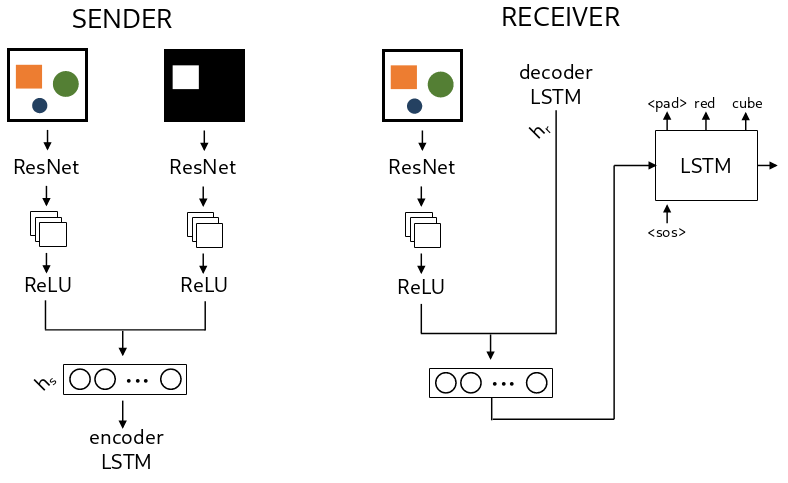
\includegraphics[width=.7\linewidth]{figures/arch_caption_generator_game.png}
    \caption{Simplified architecture of the caption generator game}
    \label{fig:caption_generator_game_architecture}
    % SD: But here we don't need an LSTM, we just want to identify one of the objects. The LSTM should only encode the inout message.
    % DK: TODO
\end{figure}

However, this setup could lead to two problems:
First, the task is quite complex for both agents to learn, since two language generation steps are involved.
This might stop the agents from converging towards a useful language.
Secondly, in case a language emerges, it could be aligned with the natural language of the target referring expressions.
In other words, the sender might just learn to effectively repeat the target referring expressions without extracting the necessary features themselves.
For that reason, in the second setup the receiver is tasked to predict only the attributes of the target object in the shape of a one-hot vector.
By this, no natural language including its salience order is involved and the complexity of the complete game is reduced.
The receiver uses the same way to encode and combine the complete scene and the sender's message with $e_{ri}=100$, $h_r=500$ and $e_r=100$.
This is then passed to a linear layer that produces a vector with 13 dimension, corresponding to the 2 sizes, 3 shapes, and 8 colors.
The loss is then calculated using binary cross entropy.

\cmtDK[inline]{figure}

The experiments for both setups are conducted with a learning rate of $2\times10^{-4}$.
As in the previous section, the following values for the variables are compared:
\begin{itemize}
    \item $|V|$: 2, 10, 16, 50, 100
    \item $n$: 1, 2, 3, 4, 6
\end{itemize}

Since the agents are trained to describe the target object discriminatively based on the described GRE-algorithm, they are trained on the \emph{Dale-2}, \emph{Dale-5} and \emph{CLEVR color} dataset.
The \emph{Dale-5} and the \emph{CLEVR color} should be again much harder to learn, since there are more objects that the agents need to discriminate the target object from.
% SD: So the sender is generating descriptions following the GRE policy?
% DK: TODO
The same metrics as in the section \ref{sec:referring_expression_generation} are used to evaluate the results for the first setup.
When predicting one-hot vectors, an overall \textbf{accuracy} is reported that reflects if all attributes were predicted correctly.
Additionally, the accuracy for each attribute is calculated separately to show which attributes give bigger challenges for the models.

\subsubsection*{Results}
\begin{table}[ht]
    \centering
    \begin{tabular}{cc|ccc|ccc|ccc}
        \toprule
                                      &        & \multicolumn{3}{c}{\textbf{Dale-2}} & \multicolumn{3}{c}{\textbf{Dale-5}} & \multicolumn{3}{c}{\textbf{CLEVR color}}                                                                                                     \\  \cmidrule(lr){3-5}\cmidrule(lr){6-8}\cmidrule(lr){9-11}
        $n$                           & $|V|$  & \textbf{Acc.}                       & \textbf{F1}                         & \textbf{NT}                              & \textbf{Acc.}    & \textbf{F1}      & \textbf{NT}     & \textbf{Acc.} & \textbf{F1} & \textbf{NT} \\\midrule
        \multicolumn{2}{c|}{baseline} & {41,8} & {42,36}                             & {37,11}                             & {62,66}                                  & {81,16}          & {18,36}          & {13,52}         & {33,08}       & {34,53}                   \\\midrule
        {1}                           & {2}    & {70,49}                             & {54,73}                             & {7,29}                                   & {70,16}          & {85,06}          & {13,06}         & {11,68}       & {32,25}     & {34,03}     \\
        {1}                           & {10}   & {78,26}                             & {63,33}                             & {3,56}                                   & {68,97}          & {85,01}          & {10,85}         & {12,72}       & {32,77}     & {33,85}     \\
        {1}                           & {16}   & {74,18}                             & {52,21}                             & {5,38}                                   & {71,57}          & {86,87}          & {10,72}         & {13,19}       & {33,64}     & {33,33}     \\
        {1}                           & {50}   & {70,83}                             & {43,56}                             & {4,21}                                   & {65,23}          & {83,11}          & {12,54}         & {11,81}       & {33,14}     & {34,72}     \\
        {1}                           & {100}  & {73,18}                             & {52,14}                             & {3,86}                                   & {60,94}          & {80,85}          & {20,36}         & {13,67}       & {33,71}     & {33,64}     \\
        {2}                           & {2}    & {72,31}                             & {50,42}                             & {5,52}                                   & {66,2}           & {83,39}          & {14,42}         & {13,32}       & {33,62}     & {32,73}     \\
        {2}                           & {10}   & {75,22}                             & {58,4}                              & {3,99}                                   & {73,22}          & {87,68}          & {9,03}          & {12,37}       & {33,3}      & {34,11}     \\
        {2}                           & {16}   & {\textbf{81,64}}                    & {\textbf{73,66}}                    & {\textbf{2,86}}                          & {73,44}          & {88,21}          & {8,85}          & {12,98}       & {33,94}     & {34,24}     \\
        {2}                           & {50}   & {74,39}                             & {48,53}                             & {3,17}                                   & {\textbf{75,35}} & {\textbf{88,77}} & {\textbf{8,07}} & {14,19}       & {33,04}     & {33,46}     \\
        {2}                           & {100}  & {74,09}                             & {54,88}                             & {3,65}                                   & {54,56}          & {76,95}          & {22,57}         & {13,28}       & {32,8}      & {33,38}     \\
        {3}                           & {2}    & {71,03}                             & {50,76}                             & {4,62}                                   & {65,18}          & {82,68}          & {14,23}         & {12,76}       & {33,58}     & {33,64}     \\
        {3}                           & {10}   & {76,91}                             & {59,42}                             & {2,6}                                    & {71,66}          & {87,14}          & {9,9}           & {12,54}       & {32,75}     & {33,85}     \\
        {3}                           & {16}   & {79,95}                             & {67,55}                             & {3,17}                                   & {50,13}          & {73,24}          & {24,22}         & {12,93}       & {33,79}     & {34,46}     \\
        {3}                           & {50}   & {62,93}                             & {48,03}                             & {16,58}                                  & {\textbf{76,09}} & {\textbf{88,5}}  & {\textbf{9,2}}  & {13,67}       & {33,73}     & {34,29}     \\
        {3}                           & {100}  & {75,74}                             & {57,51}                             & {2,43}                                   & {69,7}           & {86,14}          & {9,38}          & {13,02}       & {33,64}     & {34,2}      \\
        {4}                           & {2}    & {41,23}                             & {42,53}                             & {35,33}                                  & {63,93}          & {82,34}          & {15,3}          & {12,2}        & {33,25}     & {33,64}     \\
        {4}                           & {10}   & {78,99}                             & {66,4}                              & {2,08}                                   & {73,22}          & {88,01}          & {10,85}         & {12,5}        & {33,55}     & {33,16}     \\
        {4}                           & {16}   & {\textbf{80,08}}                    & {\textbf{70,48}}                    & {\textbf{3,47}}                          & {69,4}           & {86,09}          & {10,63}         & {11,72}       & {33,1}      & {34,03}     \\
        {4}                           & {50}   & {75,48}                             & {54,44}                             & {3,34}                                   & {71,35}          & {86,61}          & {10,68}         & {11,81}       & {33,18}     & {34,33}     \\
        {4}                           & {100}  & {74,78}                             & {57,09}                             & {3,86}                                   & {59,2}           & {80,14}          & {20,57}         & {12,67}       & {32,3}      & {34,55}     \\
        {6}                           & {2}    & {72,87}                             & {51,44}                             & {2,78}                                   & {60,82}          & {80,42}          & {17,07}         & {13,45}       & {33,73}     & {33,64}     \\
        {6}                           & {10}   & {73,61}                             & {48,73}                             & {2,82}                                   & {32,64}          & {58,42}          & {33,12}         & {11,89}       & {33,15}     & {35,03}     \\
        {6}                           & {16}   & {73,52}                             & {49,67}                             & {2,43}                                   & {49,39}          & {73,19}          & {23,78}         & {13,06}       & {32,31}     & {34,64}     \\
        {6}                           & {50}   & {44,31}                             & {45,07}                             & {33,29}                                  & {\textbf{78,82}} & {\textbf{90,22}} & {\textbf{7,29}} & {12,72}       & {33,29}     & {32,99}     \\
        {6}                           & {100}  & {\textbf{80,95}}                    & {\textbf{69,88}}                    & {\textbf{3,34}}                          & {62,2}           & {80,62}          & {19,88}         & {14,24}       & {32,36}     & {32,94}     \\
        \bottomrule
    \end{tabular}
    \caption{Overall accuracies (Acc.), F1-score (F1) and non-target accuracies (NT) in \% of the RE generator games: $n$ are different maximum message lengths and $|V|$ are different vocabulary sizes.}
    \label{tab:results:re-generator-game}
\end{table}

Table \ref{tab:results:re-generator-game} shows the \emph{overall accuracies}, \emph{F1-scores} and \emph{non-target accuracies} across all datasets for different message lengths $n$ and vocabulary sizes $|V|$.
The baselines are shown in the first row.
Hereby, the sender is sending random messages, so that the receiver needs to solve the task on their own.
In all configurations that don't pass this baseline, no meaningful messages are exchanged, and no language emerged.
If configurations perform better on the other hand means that the agents learned to encode some meaning in their messages.

When first having a look at the results of the \emph{Dale-2} dataset, it can be seen that the baseline already identifies correct referring expressions in 41,8\% of the samples.
However, almost all other configurations perform much better.
This shows that the agents consistently learn languages to solve the tasks.
Still, differences in how well the agents perform can be identified.
While a small vocabulary with $|V| = 2$ mostly beats the baseline, the emerged language only lets the agents generate the correct referring expression in a maximum of around 72\% of the samples.
The similar result is visible for a bigger vocabulary size of $|V|=50$ which has the highest accuracy at around 74\%.
A vocabulary size of $|V|=100$ performs consistently slightly better, with accuracies of around 73\% to 75\%.
Interestingly, when the agents are allowed to exchange messages with a message length of $n=6$, the accuracy peaks at almost 81\%.
Additionally, also the \emph{F1-score} almost reaches 70\% whereas it usually stayed around 50\% to 60\% in the previously discussed configuration.
The \emph{F1-score} evaluates each word in the referring expression separately instead of the binary \emph{overall accuracy} for the complete referring expression.
A small increase of the accuracy accompanied by a large increase of the F1-score indicates that the agents learned to encode an additional attribute, with the larger vocabulary and longer messages.
Finally, vocabulary sizes of $|V|=10$ and $|V|=16$ consistently perform the best with accuracies of 74\% to 81\%.
However, a difference in the \emph{F1-score} is visible: configurations with $|V|=16$ reach 67,55\% to 73,66\% with message lengths $n=[2,4]$, where $|V|=10$ only reaches an F1-score of 66,4\% with $n=4$ and otherwise performs worse.
This indicates as before that the agents were able to encode more attributes with the larger vocabulary.

The results look different when the agents are trained to generate referring expressions for the \emph{Dale-5} dataset.
First, the baseline, in other words the receiver on their own, performs much better.
It already produces the whole correct referring expressions in 62,66\% of the samples, and achieves and \emph{F1-score} of 81,36\%.
However, the \emph{non-target accuracy} is quite high with producing correct referring expressions for a distractor in 18,36\% of the cases.
This allows two conclusions: On the one side, the baseline can pretty successfully extract a bias from the images.
Since there are multiple distractors in the image, the probability that they share attributes that are relevant for discriminating the target is higher.
The model therefore can learn to generate \emph{shapes} and \emph{colors} that appear more often correctly, which leads to a higher \emph{F1-score}.
On the other side, the larger number of distractors makes it possible for the model to single out the target from the image alone, as it needs to be uniquely identifiable.
If there are for instance two large red cubes, two blue spheres, but only one green sphere, the target needs to be the green sphere, and no additional textual information is needed.
The model can exploit this bias in the dataset, which leads to a higher accuracy.
However, distractors might also be unique in the scene, so the model won't be able to consistently single out the correct unique object, which leads to a higher \emph{non-target accuracy}.
Messages by a sender would need to solve these problems.

Interestingly, many configurations with a sender perform as the baseline or even worse.
Only 16 out of 30 configurations beat the baseline, some only by a few percent points.
The best configuration however, has an accuracy of 78,82\%, an \emph{F1-score} of 90,22\% and a \emph{non-target accuracy} of 7,29\% which is 16\% points, 9\% points and 11\% points better than the baseline respectively.
The models tend to perform better with a message length of $n>1$ and $n<6$, and consistently the best across all vocabulary sizes with $n=2$.
However, there are good results for all $n$, with the best configuration utilizing $n=6$.
Looking at the vocabulary sizes, configurations with $|V|=2$ beat the baseline only slightly, except with $n=1$.
When the agents use a vocabulary with $|V|=10$, they beat the baseline consistently and push the \emph{non-target accuracy} close to and below 10\%.
However, when longer messages are allowed with $n=6$, the accuracy drops to only 32,64\%.
The reason might be that the agents learned to exchange messages about patterns that are only present in the training samples and that were not transferrable to unseen samples.
The learned language was therefore not general enough.
A similar result is visible for $|V|=16$, but the model additionally performs badly with $n=3$.
Using a vocabulary with $|V|=50$, the models can generate the best referring expressions.
Almost all configurations have an accuracy of above 70\%, three of them even above 75\%.
Having more symbols to describe the objects apparently helps the agents to learn a useful language.
However, when the bottleneck is too big, the agents are not able to encode useful messages as seen with $|V|=100$.
The agents are only able to beat the baseline with $n=3$; all other configurations perform equal or worse.

Finally, the results of the experiments with the \emph{CLEVR color} dataset show that the agents are not able to learn a language to describe the target objects.
The baseline corresponds to a random guess of the color while the other attributes are identified correctly (since they are identical for target and distractor in the complete scene).
No configuration beats this baseline which shows that no meaningful language emerges independently of vocabulary size $|V|$ and message length $n$.

\begin{table}[ht]
    \centering
    \begin{tabular}{rr|cc|c|ccc|c|c}
        \toprule
                                         &             & {small} & {large} & \textbf{size}  & {cube}  & {cylinder} & {sphere} & \textbf{shape} & {<pad>} \\\midrule
        \multirow{2}{*}{\textbf{Dale-2}} & {Precision} & {45,15} & {37,96} & \textbf{41,56} & {99,25} & {99,65}    & {99,21}  & \textbf{99,37} & {94,58} \\
                                         & {Recall}    & {16,69} & {6,23}  & \textbf{11,46} & {99,59} & {98,55}    & {99,84}  & \textbf{99,33} & {99,3}  \\\midrule
        \multirow{2}{*}{\textbf{Dale-5}} & {Precision} & {80,9}  & {89,63} & \textbf{85,27} & {97,67} & {97,7}     & {95,21}  & \textbf{96,86} & {88,1}  \\
                                         & {Recall}    & {76,99} & {69,14} & \textbf{73,07} & {96,58} & {97,22}    & {96,72}  & \textbf{96,84} & {96,1}  \\\midrule
        \multirowcell{2}[0pt][r]{\textbf{CLEVR}                                                                                                          \\\textbf{color}} & {Precision}  & {-}     & {-}     & \textbf{-}     & {100}   & {100}      & {100}    & \textbf{100}   & {100}   \\
                                         & {Recall}    & {-}     & {-}     & \textbf{-}     & {100}   & {100}      & {100}    & \textbf{100}   & {100}   \\
        \bottomrule
    \end{tabular}
    \caption{Precision and Recall in \% for <pad>, size and shape tokens for the configurations with the highest accuracy in Table \ref{tab:results:re-generator-game}. The columns \textbf{shape} and \textbf{size} show the average across all tokens of the respective attribute.}
    \label{tab:results:re-generator-game_size-shape}
\end{table}

\begin{table}[ht]
    \centering
    \begin{tabular}{rr|cccccccc|c}
        \toprule
                                         &             & {blue}  & {brown} & {cyan}  & {gray}  & {green} & {purple} & {red}   & {yellow} & \textbf{color}   \\\midrule
        \multirow{2}{*}{\textbf{Dale-2}} & {Precision} & {66}    & {79,35} & {71,14} & {86,11} & {70,48} & {70,74}  & {67,95} & {76,26}  & \textbf{73,5}    \\
                                         & {Recall}    & {88,96} & {63,43} & {91,9}  & {46,02} & {69,29} & {65,99}  & {75,35} & {79,54}  & \textbf{72,56}   \\\midrule
        \multirow{2}{*}{\textbf{Dale-5}} & {Precision} & {92,61} & {93,3}  & {94,73} & {91,12} & {93,66} & {88,71}  & {88,04} & {89,79}  & \textbf{91,5}    \\
                                         & {Recall}    & {89,09} & {86,31} & {91,08} & {89,08} & {83,23} & {92,16}  & {93,05} & {88,77}  & {\textbf{89,1}}  \\\midrule
        \multirowcell{2}[0pt][r]{\textbf{CLEVR}                                                                                                             \\\textbf{color}} & {Precision}           & {0} & {0} & {0} & {0} & {12,91} & {13,9}  & {0} & {0}   & \textbf{3,35} \\
                                         & {Recall}    & {0}     & {0}     & {0}     & {0}     & {36,25} & {69,85}  & {0}     & {0}      & {\textbf{13,26}} \\
        \bottomrule
    \end{tabular}
    \caption{Precision and Recall in \% for color tokens for the configurations with the highest accuracy in Table \ref{tab:results:re-generator-game}. The column \textbf{color} shows the average across all colors.}
    \label{tab:results:re-generator-game_color}
\end{table}

Tables \ref{tab:results:re-generator-game_size-shape} and \ref{tab:results:re-generator-game_color} show the precision and recall divided by attributes and tokens.
The results have a similar general pattern to the single model experiments in Section \ref{sec:referring_expression_generation}.
For the \emph{Dale} dataset, the \emph{shape} is identified well while the agents struggle more with the \emph{color} and the most with the \emph{size}.
The agents identify the \emph{shape} and \emph{size} perfectly on the \emph{CLEVR color} dataset, but only predict few \emph{colors}.

Looking at the \emph{shape}, the agents perform almost perfectly with the \emph{Dale-2} dataset.
The precision and recall are slightly lower with the \emph{Dale-5} dataset, and the agents predict the \emph{sphere} too often, while predicting the \emph{cube} too few.
The difference however lies only around 1\%.

Interestingly, the agents can predict the \emph{color} the best, when presented with the \emph{Dale-5} dataset.
The precision and recall lie around 90\%, while for the \emph{Dale-2} dataset they lie only around 73\%.
However, there is a bigger difference across the colors.
Some colors are predicted more often (e.g. purple and red for \emph{Dale-5}, and yellow red, cyan and blue for \emph{Dale-2}) than others (e.g. brown and green for \emph{Dale-5}, and purple, gray and brown for \emph{Dale-2}).
As can be seen, the colors are not consistent and "difficult" or "easy" colors can't be identified.
Additionally, these colors also differ across several runs of the same configurations and datasets.
The differences between the two \emph{Dale} dataset, might be explainable by the number of scenes in which the color is part of the referring expression.
As seen in Table \ref{tab:results:re-generator-game}, the \emph{overall accuracy} is higher for the \emph{Dale-2} dataset, even though the prediction of the \emph{color} attribute is worse.
The reason for this is that many referring expressions in the \emph{Dale-2} dataset only rely on the \emph{shape} and no \emph{color} is needed.
The agents therefore can perform well even though predictions of the \emph{color} are wrong.
On the other side, the \emph{color} is a central part of almost all referring expressions in the \emph{Dale-5} dataset and the agents are pushed to learn this attribute more intensely.

Since the single model in section \ref{sec:referring_expression_generation} already struggled with predicting the \emph{color} on the \emph{CLEVR color} dataset, it is no surprise that it performs badly in the more complex setup of language games.
Hereby, the agents are not able to communicate anything and the receiver only generates two colors (green and purple) for all shown samples.
This results in a random guess of one of the 8 \emph{colors}, explaining the \emph{overall accuracy} of $\frac{1}{8}=12,5\%$.

The final attribute is the \emph{size}.
While the agents easily learn that the \emph{size} is never part of the referring expression for the \emph{CLEVR color} dataset, they struggle with the \emph{Dale} datasets.
As in section \ref{sec:referring_expression_generation}, the agents again struggle to predict the correct length of the referring expression.
Especially, the agents predict too short referring expressions as the precision of the \emph{<pad>} token in lower than its recall.
This is mostly due to the \emph{size} attribute, since a large difference of the precision and recall is visible.
As for the \emph{color}, the agents perform better on the \emph{Dale-5} dataset.
This reason might be the same.
The \emph{size} attribute is more often needed to discriminate the target object and appears therefore in more samples and is more central in the referring expressions.
Similarly to the \emph{color} attribute, there are differences between the single tokens.
However, these are not constant across configurations, datasets and runs and no "difficult" token can be identified.

\begin{table}[ht]
    \centering
    \begin{tabular}{cc|ccc|ccc|ccc}
        \toprule
                                      &         & \multicolumn{3}{c}{\textbf{Dale-2}} & \multicolumn{3}{c}{\textbf{Dale-5}} & \multicolumn{3}{c}{\textbf{CLEVR colour}}                                                                                                                                                                                                           \\  \cmidrule(lr){3-5}\cmidrule(lr){6-8}\cmidrule(lr){9-11}
        $n$                           & $|V|$   & \textbf{A\textsubscript{color}}     & \textbf{A\textsubscript{shape}}     & \textbf{A\textsubscript{size}}            & \textbf{A\textsubscript{color}} & \textbf{A\textsubscript{shape}} & \textbf{A\textsubscript{size}} & \textbf{A\textsubscript{color}} & \textbf{A\textsubscript{shape}} & \textbf{A\textsubscript{size}} \\\midrule
        \multicolumn{2}{c|}{baseline} & {92,03} & {88,91}                             & {50,55}                             & {89,38}                                   & {80,78}                         & {49,92}                         & {90,78}                        & {100}                           & {76,72}                                                          \\\midrule
        {1}                           & {2}     & {93,68}                             & {89,69}                             & {52,04}                                   & {90,12}                         & {88,09}                         & {49,74}                        & {87,37}                         & {100}                           & {76,56}                        \\
        {1}                           & {10}    & {94,21}                             & {96,31}                             & {52,78}                                   & {90,15}                         & {90,6}                          & {49,74}                        & \textbf{91,32}                  & {100}                           & {76,52}                        \\
        {1}                           & {16}    & {92,8}                              & {94,97}                             & {52,78}                                   & {93,45}                         & {91,97}                         & {49,74}                        & {91,03}                         & {100}                           & {76,52}                        \\
        {1}                           & {50}    & {91,58}                             & {90,1}                              & {52,78}                                   & {93,39}                         & {94,66}                         & {49,74}                        & {89,41}                         & {100}                           & {76,52}                        \\
        {1}                           & {100}   & {92,66}                             & {90,41}                             & {52,78}                                   & {90,23}                         & {83,03}                         & {49,74}                        & {86,72}                         & {100}                           & {76,52}                        \\
        {2}                           & {2}     & {92,45}                             & {92,45}                             & {52,04}                                   & \textbf{94,38}                  & {88,72}                         & {49,74}                        & {88,89}                         & {100}                           & {76,56}                        \\
        {2}                           & {10}    & {\textbf{94,44}}                    & {96,09}                             & {52,78}                                   & {90,71}                         & {91,54}                         & {49,74}                        & {89,54}                         & {100}                           & {76,52}                        \\
        {2}                           & {16}    & {92,66}                             & {90,58}                             & {52,78}                                   & {94,14}                         & \textbf{97,18}                  & {49,74}                        & {86,98}                         & {100}                           & {76,52}                        \\
        {2}                           & {50}    & {92,45}                             & {89,28}                             & {52,78}                                   & {93,01}                         & {92,01}                         & {49,74}                        & {86,5}                          & {100}                           & {76,52}                        \\
        {2}                           & {100}   & {92,97}                             & {\textbf{98,91}}                    & {52,78}                                   & {92,49}                         & {92,66}                         & {49,74}                        & {86,68}                         & {100}                           & {76,52}                        \\
        {3}                           & {2}     & {93,32}                             & {90,97}                             & {52,04}                                   & {92,53}                         & {87,88}                         & {49,74}                        & {90,58}                         & {100}                           & {76,56}                        \\
        {3}                           & {10}    & \textbf{{94,79}}                    & {97,01}                             & {52,78}                                   & {92,8}                          & {94,4}                          & {49,74}                        & \textbf{91,17}                  & {100}                           & {76,52}                        \\
        {3}                           & {16}    & {93,1}                              & {95,36}                             & {52,78}                                   & {91,88}                         & {86,72}                         & {49,74}                        & {88,06}                         & {100}                           & {76,52}                        \\
        {3}                           & {50}    & {90,84}                             & {90,93}                             & {52,78}                                   & \textbf{94,18}                  & {94,92}                         & {49,74}                        & {88,59}                         & {100}                           & {76,52}                        \\
        {3}                           & {100}   & {90,76}                             & {89,37}                             & {52,78}                                   & {92,8}                          & {94,1}                          & {49,74}                        & \textbf{91,84}                  & {100}                           & {76,52}                        \\
        {4}                           & {2}     & {92,11}                             & {94,86}                             & {52,04}                                   & {93,86}                         & {88,56}                         & {49,74}                        & {87,11}                         & {100}                           & {76,56}                        \\
        {4}                           & {10}    & {92,75}                             & {90,58}                             & {52,78}                                   & {93,71}                         & {95,05}                         & {49,74}                        & {89,89}                         & {100}                           & {76,52}                        \\
        {4}                           & {16}    & {94,14}                             & {\textbf{98,57}}                    & {52,78}                                   & {\textbf{95,23}}                & \textbf{96,14}                  & {49,74}                        & {88,06}                         & {100}                           & {76,52}                        \\
        {4}                           & {50}    & {93,32}                             & {95,66}                             & {52,78}                                   & {90,45}                         & {91,01}                         & {49,74}                        & {88,85}                         & {100}                           & {76,52}                        \\
        {4}                           & {100}   & {93,58}                             & {89,41}                             & {52,78}                                   & {93,19}                         & {94,66}                         & {49,74}                        & {86,98}                         & {100}                           & {76,52}                        \\
        {6}                           & {2}     & {92,94}                             & {93,39}                             & {52,04}                                   & {92,16}                         & {82,18}                         & {49,74}                        & {90,05}                         & {100}                           & {76,56}                        \\
        {6}                           & {10}    & {\textbf{94,23}}                    & {\textbf{98,78}}                    & {52,78}                                   & {92,75}                         & \textbf{96,79}                  & {49,74}                        & {87,67}                         & {100}                           & {76,52}                        \\
        {6}                           & {16}    & {91,32}                             & {96,96}                             & {52,78}                                   & {93,75}                         & {95,57}                         & {49,74}                        & {89,37}                         & {100}                           & {76,52}                        \\
        {6}                           & {50}    & {91,45}                             & {88,28}                             & {52,78}                                   & {86,24}                         & {91,71}                         & {49,74}                        & {88,32}                         & {100}                           & {76,52}                        \\
        {6}                           & {100}   & {92,45}                             & {94,92}                             & {52,78}                                   & {93,62}                         & {95,3}                          & {49,74}                        & {89,19}                         & {100}                           & {76,52}                        \\
        \bottomrule
    \end{tabular}
    \caption{Accuracies for each attribute in \% of the attribute predictor games: $n$ are different maximum message lengths and $|V|$ are different vocabulary sizes.}
    \label{tab:results:attribute-predictor-game}
\end{table}

Finally, Table \ref{tab:results:attribute-predictor-game} show the results for the games in which the receiver predicts a one-hot vector of the attributes.
Again, the baselines are games, the receiver plays alone.
Hereby, it can be seen that the receiver can already predict the \emph{color} and \emph{shape} very well: 92\% and 88,91\% respectively on the \emph{Dale-2} dataset, 89,38\% and 80,78\% respectively on the \emph{Dale-5} dataset, and 90,78\% and 100\% respectively on the \emph{CLEVR color} dataset.
The \emph{size} however corresponds to a random guess on the \emph{Dale} dataset and only achieves 76,72\% on the \emph{CLEVR color} dataset.


\begin{table}[ht]
    \centering
    \begin{tabular}{ccc|ccc|ccc}
        \toprule
              &         &         & \multicolumn{3}{c}{\textbf{Dale-2}} & \multicolumn{3}{c}{\textbf{Dale-5}}                                                                             \\\cmidrule(lr){4-6}\cmidrule(lr){7-9}
        $|V|$ & $h_{s}$ & $h_{r}$ & \textbf{Acc.}                       & \textbf{word-by-word}               & \textbf{length} & \textbf{Acc.} & \textbf{word-by-word} & \textbf{length} \\\midrule
        {10}  & {10}    & {10}    & {22,9\%}                            & {62,8\%}                            & {1}             & {7,1\%}       & {40\%}                & {1}             \\
        {13}  & {10}    & {10}    & {22,8\%}                            & {62,9\%}                            & {0}             & {7,3\%}       & {38,7\%}              & {1}             \\
        {20}  & {10}    & {10}    & {24,6\%}                            & {64\%}                              & {1}             & {6,7\%}       & {38,7\%}              & {1}             \\
        {100} & {10}    & {10}    & {24,4\%}                            & {62\%}                              & {1}             & {7,8\%}       & {40\%}                & {1}             \\
        {100} & {100}   & {100}   & {21\%}                              & {62\%}                              & {1}             & {6,5\%}       & {37,8\%}              & {1}             \\
        \bottomrule
    \end{tabular}
    \caption{Results of the caption generator: $|V|$ are different vocabulary sizes and $h$ hidden sizes.}
    % SD: What is word-by-word?
    % DK: the same as in the caption generator with a single model (QUESTION)
    \label{tab:results_caption_generator_game}
\end{table}

The results of the caption generator game are summarized in Table \ref{tab:results_caption_generator_game}.
In general, it can be seen that the agents have much bigger problems, to solve the task together than a single neural network.
The highest accuracy for descriptions, the agents manage to predict correctly is at 24,6\% for images of the 'Dale-2' dataset.
Compared to the (masked) accuracy of the single model with 72\%, the agents predict 47,4\% points less correct descriptions.
A similar worse performance can be seen for the 'Dale-5' dataset.
Here, the agents only manage to produce for 7,8\% of the images correct descriptions with a vocabulary size of 100, 13,2\% points less than the single neural model.
The same effect can be seen for the word-by-word accuracy, which is much lower than the metric for the single neural model for both datasets.
% SD: With the vocabulary size of 100.
% DK: (done)

When looking, how the different variables affect the performance, it can be seen that a bigger vocabulary size tends to help the agents.
% SD: Not sure. The difference is still very small, within a couple of %.
% DK: TODO
This is only visible for the 'Dale-2' dataset.
With constant hidden sizes of 10, the agents score around 22,9\% with only 10 and 13 available symbols.
When this is increased to 20 and respectively 100 symbols, the agents can increase their accuracy to around 24,5\%.
However, the increase is relatively small.
Interestingly, this effect only occurs, when the hidden sizes are small with only 10 dimensions.
As soon as they are increased to 100 dimensions with a vocabulary size of 100 symbols, the accuracy drops to 21\%.
% SD: Very small decerase for such a large difference in vocabulary size compared to what we have seen earlier.
% DK: TODO

Looking at the 'Dale-5' dataset, the increase is still there, when the vocabulary is increased to 100 symbols.
Nonetheless, the difference is with 0,5\% points even smaller and the reason may be due to other influences, such as the random initialization of the weights of the agents.
This is confirmed, when looking at emerged languages.
In all the setups, the same message is communicated for all samples, independently of the input image.
This is also reflected in the length of the messages.
For the setup with a vocabulary size of $|V| = 13$, no message is transferred, and the accuracy stays the same as in the other setups.
% SD: Here it would be much better to have a loss curve to show differences in loss between the number of communication events, the same could also be done for accuracy. Then we would have a clearer picture of how vocabulary size affects learning. It could be that with 100 vocabulary there is actually a better performance than before the final cut-off point. Is this possible? How was the final cut-off point determined anyway?
% DK: TODO

These results show that the agents are not at all able to encode meaning about the images and target objects in their messages.
% SD: Negative result: how can we then interpret that? What could we change? What did we learn from this?
% DK: TODO
This is especially interesting, compared to single model caption generator in section \ref{sec:referring_expression_generation}.
In these experiments, the model was able to converge towards correct captions and therefore able to extract the necessary information.
This shows that a main challenge for the agents lies in grounding symbols in these extracted features.
